\chapter{Analiza danych Big Data}

Termin \textit{Big Data} odnosi się do dużych, zmiennych i różnorodnych zbiorów danych, których przetwarzanie i analiza jest pracochłonne, ale może prowadzić do ciekawych wniosków oraz pozyskania nowej wiedzy. Zbieranie oraz przechowywanie dużej ilości danych do analizy było praktykowane od bardzo dawna, jednak dokładniejsza koncepcja Big Data została poznana w 2001 roku kiedy to analityk Doug Laney zaprezezentował znaną dzisiaj definicję \textit{3V}: \textit{volume}, \textit{velocity}, \textit{variety} czyli: ilość, szybkość, złożoność, a później dodano jeszcze czwarty atrybut \textit{veracity} czyli: wiarygodność.

\section{Pojęcie Big Data}
Wraz ze wzrostem zainteresowania Big Data podjęto próby dokładniejszego opisania tego terminu. Obecnie definiując to pojęcie trzeba odnieść się do nowych rozwiązań technologicznych dotyczących wielkich wolumenów danych o innym charakterze ilościowym oraz jakościowym niż dotychczas. \\
Jedna z pierwszych definicji Big Data została zaprezentowana przez M. Cox i D. Ellsworth w 1997 r. jako duża ilość danych, którą należy zwiększać, aby wydobyć wartości informacyjne. Inna i najbardziej popularna, została przestawiona w 2001 r. przez pracującego dla firmy analityczno-doradczej wspomnianego analityka D. Laney, opiera się o trzy atrybuty: ilość, szybkość i złożoność. W 2012 r. ta sama firma dodała do swojej definicji kolejne dwa atrybuty: zmienność i złożoność. Autorzy innej publikacji \textit{Big Data: Issues, Challenges, Tools and Good Practices} z 2013 r. definiują pojęcie Big Data jako wymagające stosowania nowych technologii i architektur z powodu potrzeby ekstrakcji wartości płynącej z tych danych. \\
Podsumowując, określenie Big Data to pojęcie odnoszące się do zbiorów danych, które jednocześnie charakteryzują się dużą objętością, różnorodnością, strumieniowym napływem w czasie rzeczywistym, zmiennością, złożonością oraz wymagają stosowania innowacyjnych technologii i narzędzi, aby możliwe było wydobycie z nich wartościowych informacji.

\begin{figure}[h] % h means here
	\centering
	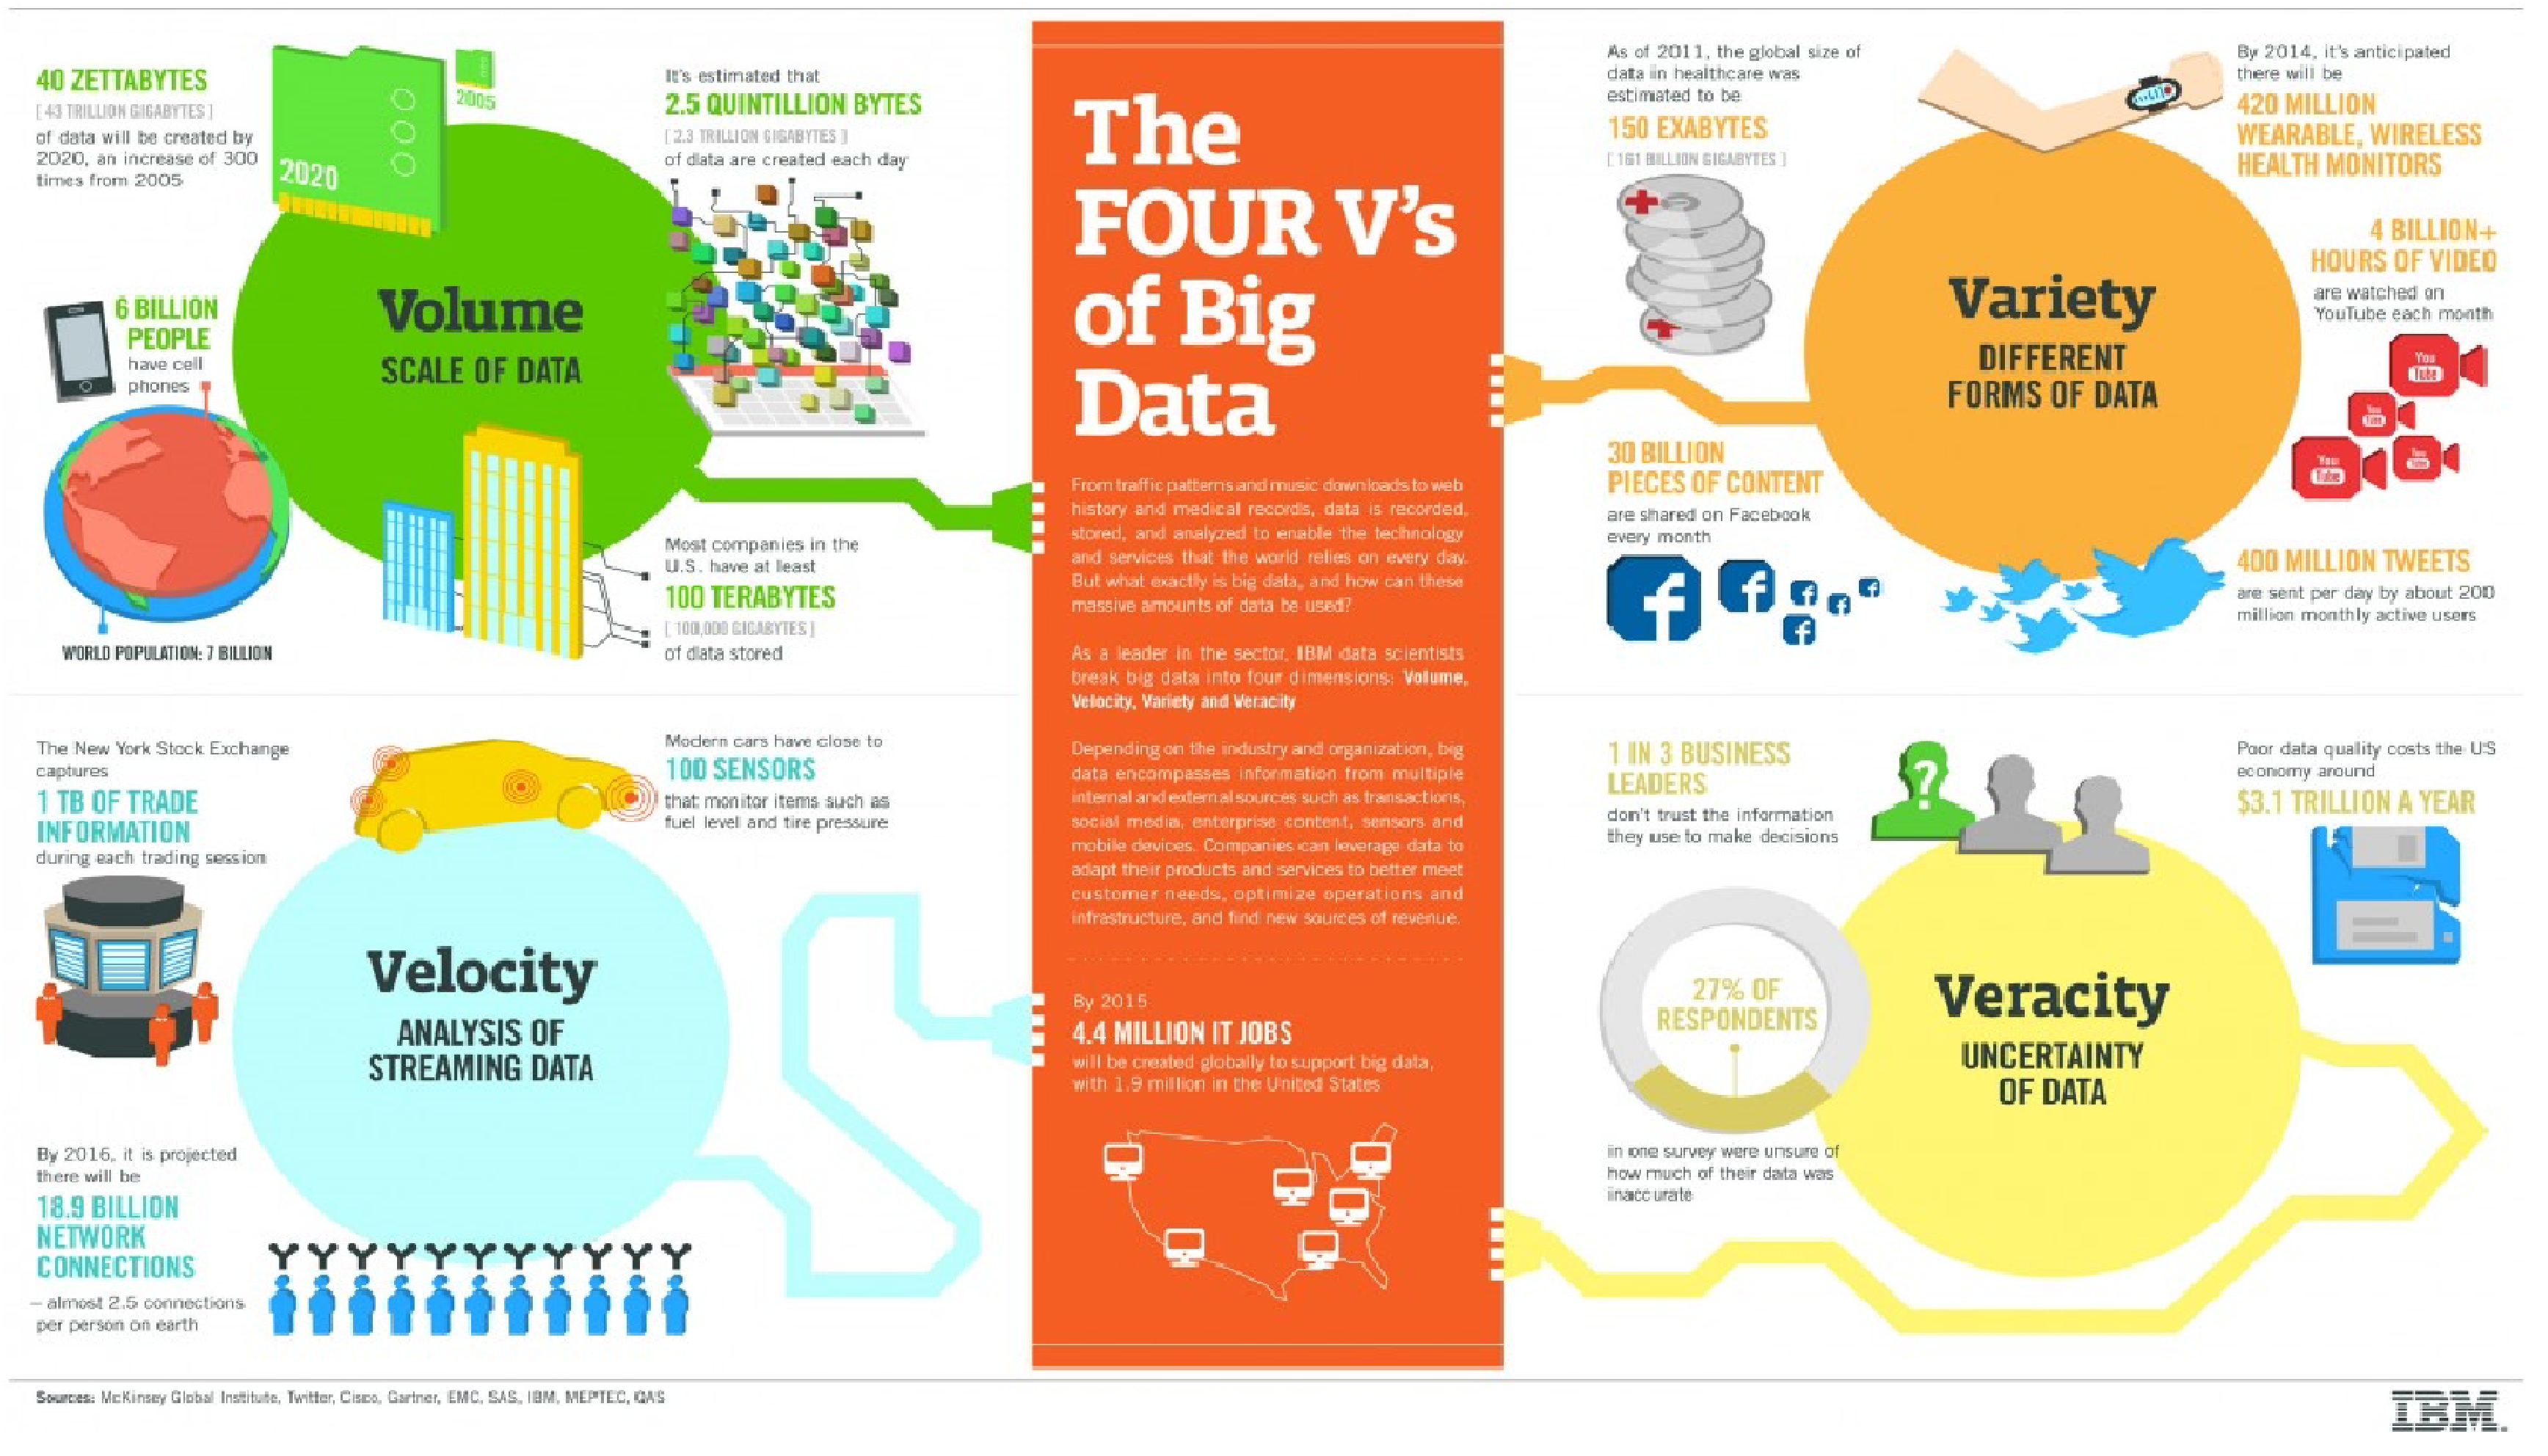
\includegraphics[width=1.0\linewidth]{img/big_data_4_v}
	\caption{Definicja \textit{Big Data} w ujęciu 4V.}
\end{figure}

\section{Charakterystyka}
Termin Big Data charakteryzują atrybuty: objętość, szybkość, różnorodność, zmienność, złożoność i wartość. W dalszej cześci tej pracy dyplomowej przedstawiono omówienie każdego z tych atrybutów.

\subsection{Objętość}
Atrybut ten odnosi się do dużej ilości danych, które wymagają nowych technologii. Rozmiar danych zależy od dziedziny i może wynosić od terabajtów lub petabajtów w zagadnieniach takich jak np. analiza zderzeń cząstek elementarnych w fizyce do megabajtów lub gigabajtów np. w telekomunikacji przy analizie połączeń wykonywanych przez abonentów. Najnowsze badania prognozują, że ilość danych wzrośnie do 2020 r. o 40\% zeta bajtów, co będzie skutkować 50-krotnym wzrostem od początku 2010 r..